\begin{frame}

\frametitle{Git: Introduction}

\begin{block}{Git}
Distributed CVS which provides the users with the ability to track the changes of files. 
\end{block}

\begin{figure}
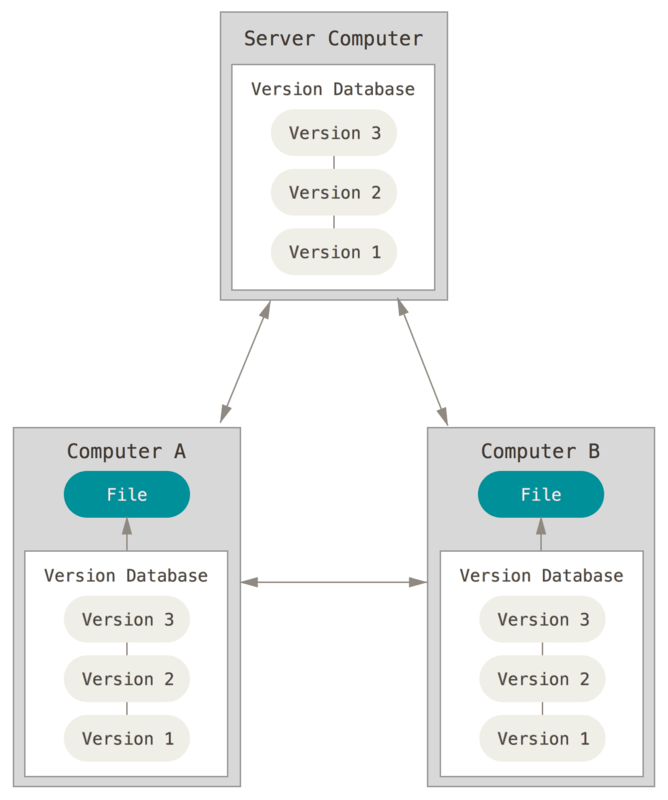
\includegraphics[scale=0.15]{distributed.png}
\caption{Distributed VCS. From \href{https://git-scm.com/book/en/v2/Getting-Started-About-Version-Control}{Git SCM}}
\label{fig:distributed}
\end{figure}

\end{frame}

\begin{frame}

\frametitle{Git: Introduction}

Also provides the following features:
\begin{itemize}
\item Branching (git branch)
\item Version merging (git merge)
\item Change rearrangement (git rebase)
\item Undoing changes
\item Tagging changes (git tag)
\item MANY more
\end{itemize}

\end{frame}

\begin{frame}[fragile]

\frametitle{Git: Introduction}

To start a git repo from scratch you shall have installed Git package. 

Besides that, go to the desired directory and type the following:

\begin{lstlisting}[language=Bash]
git init
\end{lstlisting}

After that, you can start creating and modifying files under Git.

If you already have a existing repo you can clone the remote repo typing:

\begin{lstlisting}[language=Bash]
git clone <repo_url>
\end{lstlisting}

\end{frame}
